%%
% Please see https://bitbucket.org/rivanvx/beamer/wiki/Home for obtaining beamer.
%%
\documentclass[xcolor=dvipsnames]{beamer} 
\usepackage{graphicx}
\usetheme{Frankfurt}
\setbeamertemplate{items}[circle]
\setbeamertemplate{bibliography item}[text]

% Auto creates the dots for each slide in a section
\usepackage{remreset}
\makeatletter
\@removefromreset{subsection}{section}
\makeatother
\setcounter{subsection}{1}
%\usepackage{dsfont}
%\usepackage{amsmath}
%\usepackage{amssymb}
%\usepackage{amsfonts} 
%\usepackage{mathtools}
%\usepackage{graphicx}
%\usepackage{bm}
%\usepackage{subcaption}
%\usepackage{fancyvrb}
%\usepackage{subfigure}
%\usepackage{graphicx,xcolor}
%\usepackage{pifont,mdframed}
\usepackage{tikz}
\usepackage{bm}
\usetikzlibrary{fit,positioning}

\newcommand \wdoc  { { \boldsymbol{w}_d      } }
\newcommand \wdn   { { \boldsymbol{w}_{dn}   } }
\newcommand \thd   { { \boldsymbol{\theta}_d } }
\newcommand \zdn   { { \boldsymbol{z}_{dn}   } }
\newcommand \zdnk  { { z_{dnk}           } }
\newcommand \ydm   { { \boldsymbol{y}_{dm}   } }
\newcommand \ydmk  { { y_{dmk}           } }
\newcommand \ldoc  { { \boldsymbol{l}_d      } }
\newcommand \vocab { { \boldsymbol{beta}_k   } }
\newcommand \phd   { { \boldsymbol{\phi}_d   } }

\newcommand \nor[2]    { { \mathcal{N}\left(#1, #2 \right) } }
\newcommand \muln[2]   { { \mathcal{M}\left(#1, #2 \right) } }
\newcommand \mulone[1] { { \mathcal{M}\left(#1, 1 \right)  } }
\newcommand \dir[1]    { { \mathcal{D}\left(#1 \right)     } }
\newcommand \mnor[3]   { { \mathcal{N}\left(#1, #2, #3 \right)  } }

\newcommand \alphav  { { \boldsymbol{\alpha}  } }
\newcommand \betav   { { \boldsymbol{\beta}   } }
\newcommand \lambdav { { \boldsymbol{\lambda} } }
\newcommand \vv[1]   { { \boldsymbol{#1} } }
\newcommand \T       { { ^\top } }
\newcommand \one     { { \boldsymbol{1} } }
\newcommand \vecf[1] { { \text{vec}\left( #1 \right)  } }
\newcommand \diag[1] { { \text{diag}\left( #1 \right) } }
\newcommand \lse[1]  { { \text{lse}\left( #1 \right)  } }
\newcommand \ex[2]   { { \mathbb{E}_{{#1}}\left[ #2 \right] } }

\newcommand \xid { { \boldsymbol{\xi}_d } }

\newcommand \mtd { { \boldsymbol{m}_d^{\Theta} } }
\newcommand \std { { S_d^{\Theta}              } }
\newcommand \mpd { { \boldsymbol{m}_d^{\Phi}   } }
\newcommand \spd { { S_d^{\Phi}                } }

\newcommand \thdo { { \Theta_{d\cdot}  } }
\newcommand \thok { { \Theta_{\cdot k} } }
\newcommand \phdo { { \Phi_{d\cdot}    } }
\newcommand \phok { { \Phi_{\cdot k}   } }

\newcommand \MReal[2] { { \mathbb{R}^{#1 \times #2}  } }
\newcommand \Tr[1]    { { \text{tr}\left( #1 \right) } }
\newcommand \invb[1]  { { \left( #1 \right)^{-1}     } }





\author{Bryan Feeney} 
\title{Recommending Academic Papers}
\institute[Amazon]{
 Amazon Interview Presentation
}
\date[November 22, 2017]{November 22, 2017}

\begin{document}

%--- the titlepage frame -------------------------%


\begin{frame}[plain]
  \titlepage
\end{frame}




%--- Research - MTL -------------------------%


\section{Introduction}
\begin{frame}{Introduction}

Prediction of Out-Links for Academic Papers

\begin{itemize}
    \item Background
    \item Model \& Inference
    \item Evaluation
    \item Conclusions \& Further Work
\end{itemize}


\end{frame}

%--- Background ----------------------------------%

\section{Background}

\begin{frame}{Paper Link Structure}

\begin{center}
\only<1> {
    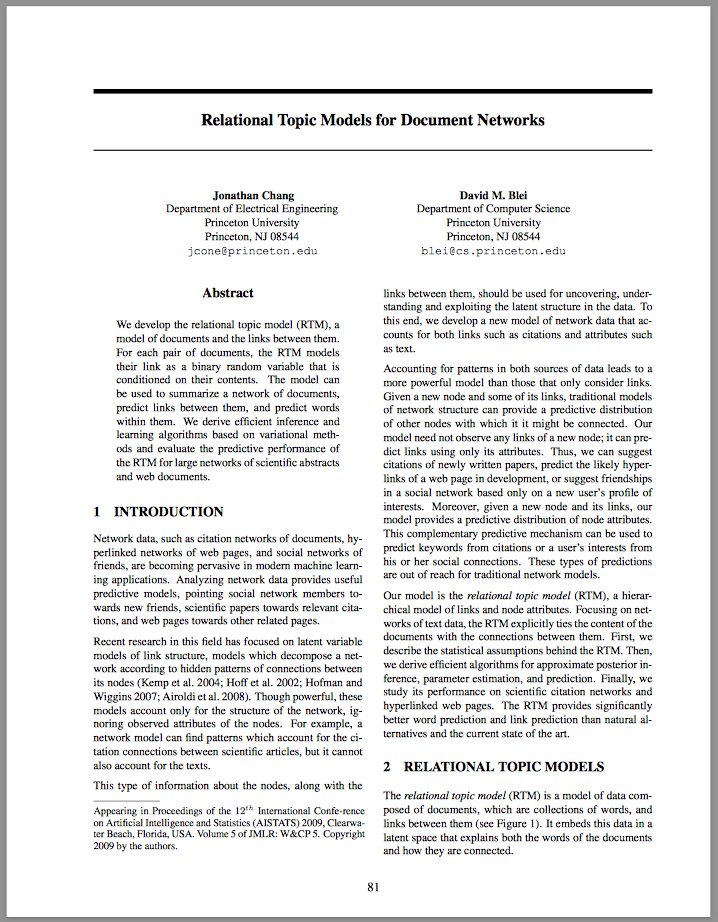
\includegraphics[scale=0.2]{rtm-frontpage.png}
    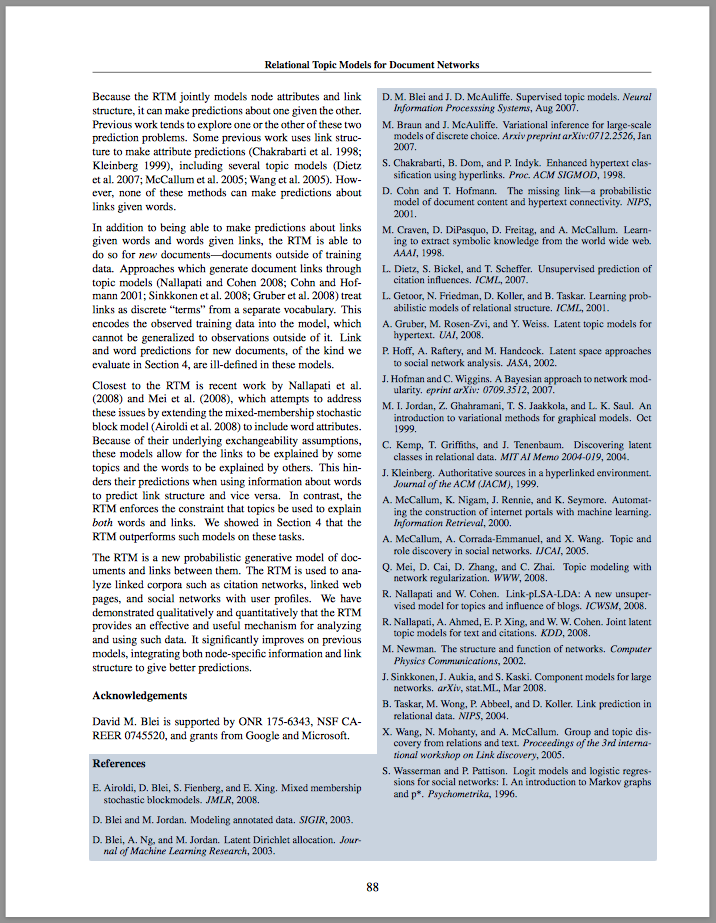
\includegraphics[scale=0.2]{rtm-citations.png}  }
\only<2> {
    
\includegraphics[scale=0.4]{doc_links_doc.pdf}
}
\only<3> {
    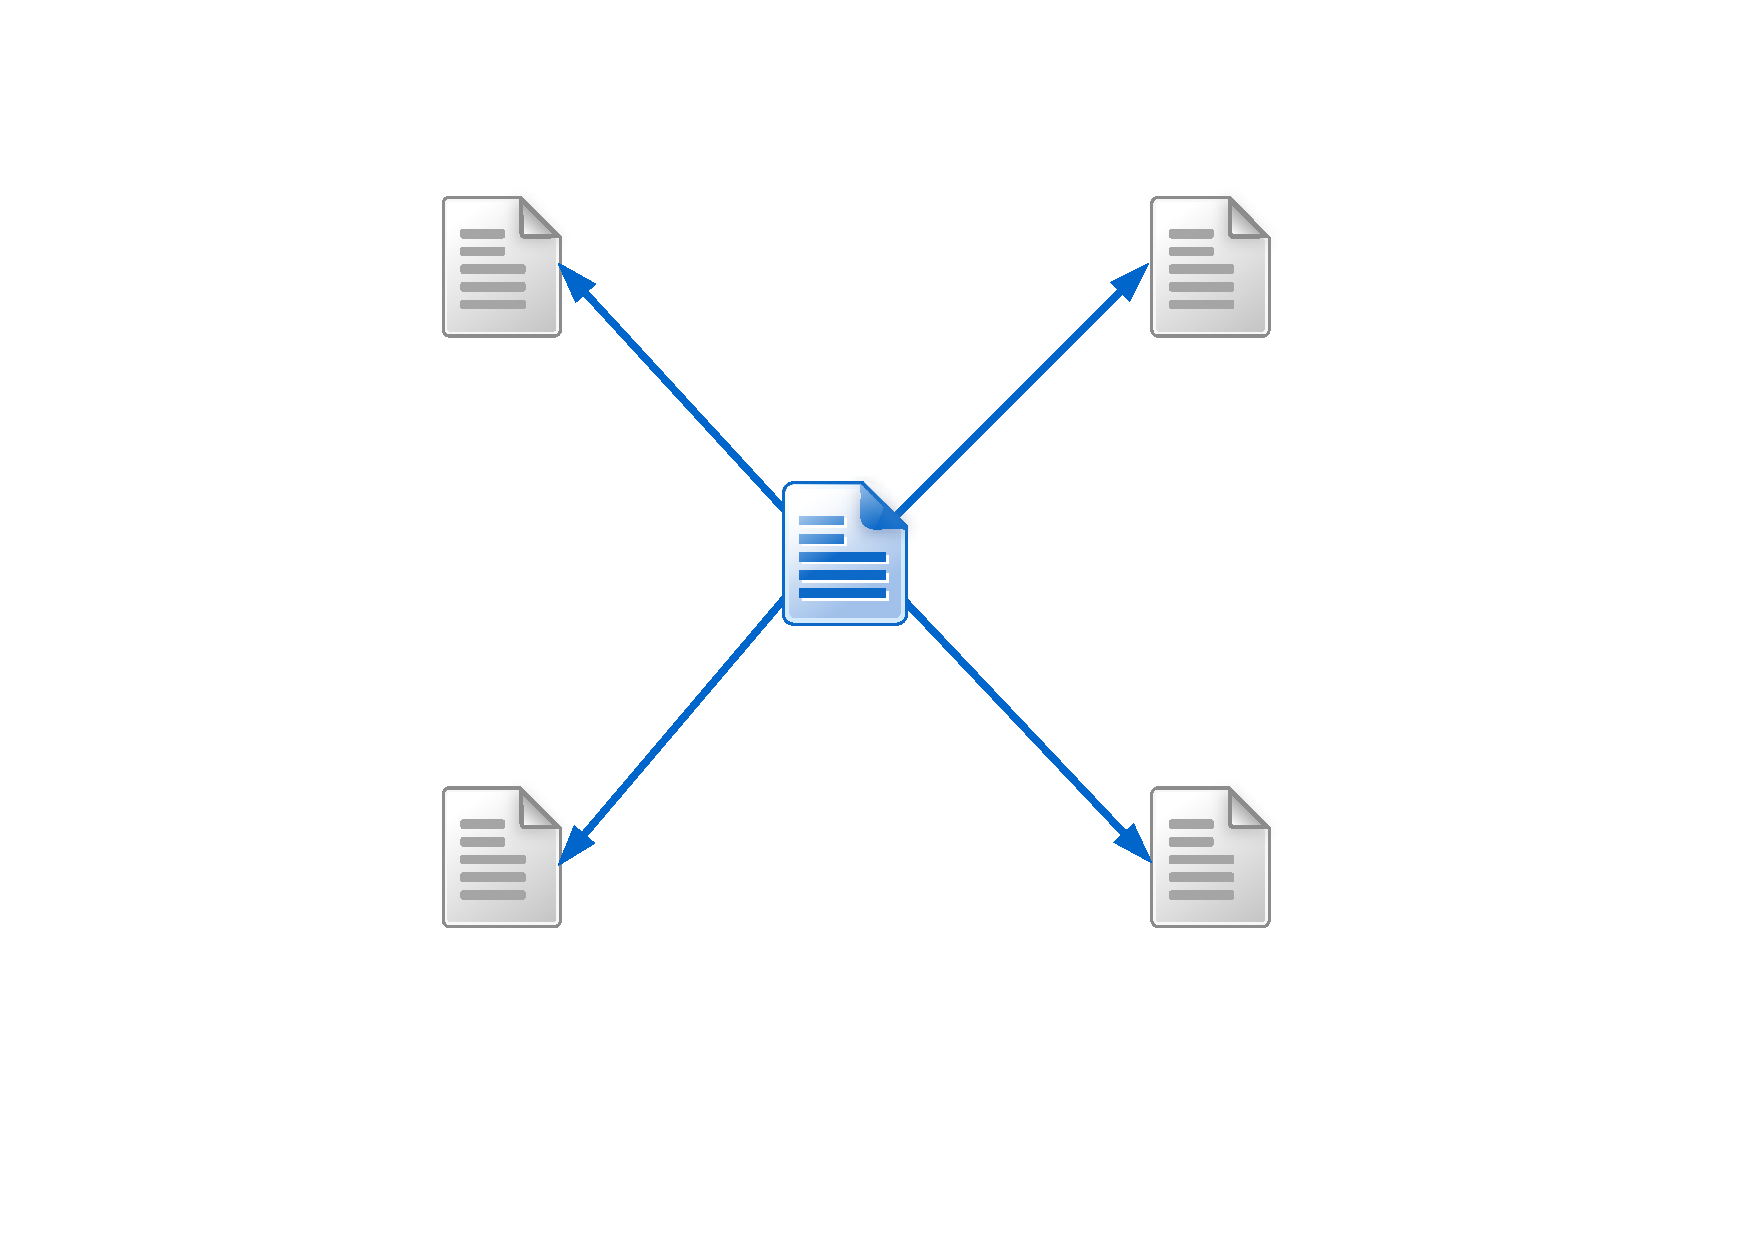
\includegraphics[scale=0.4]{doc_links_out.pdf}
}
\only<4> {
    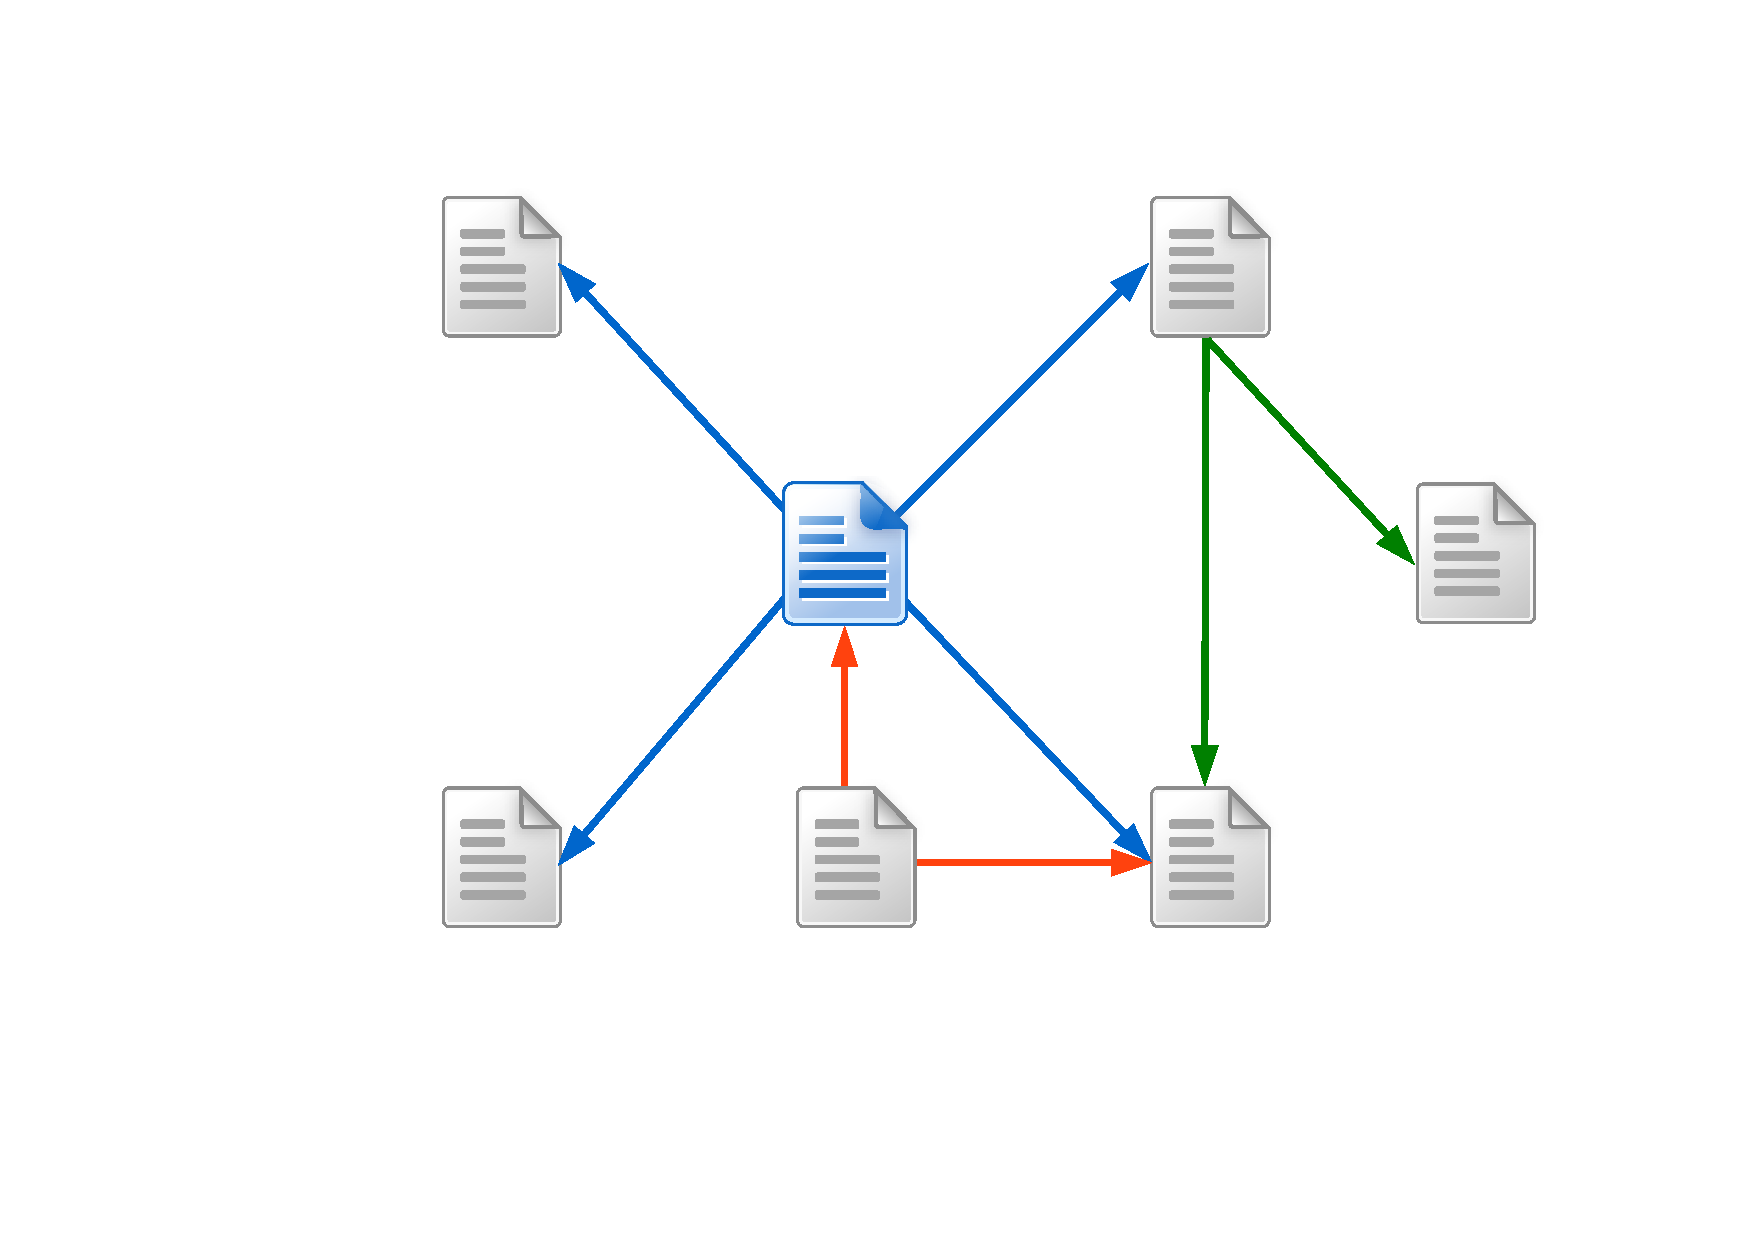
\includegraphics[scale=0.4]{doc_links_in_out.pdf}
}
\end{center}

\end{frame}

\begin{frame}{Paper Link Structure}

\only<1> {
    Topic Models\cite{BleiNgJordan2003}\cite{Buntine2014}
    \medskip
    \begin{center}
        \resizebox{0.4\textwidth}{0.20\textwidth}{
            %\documentclass{standalone}
%\usepackage{amsmath}
%\usepackage{tikz}
%\usepackage{xcolor}
%\usetikzlibrary{fit,positioning}
%\begin{document}

% ---------------------------------------------------
% Comment above for inclusion in other docs
% ---------------------------------------------------


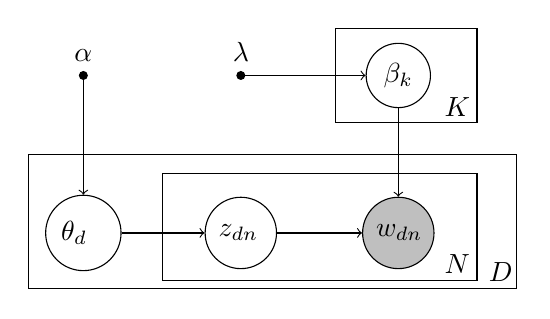
\begin{tikzpicture}
\coordinate (alpha)   at (0,2);
\node (alpha) at (0,2) [circle, draw, inner sep=1pt, fill, label=above:$\alpha$] { };
\node (theta) at (0,0) [circle, draw, text width = 16pt] {$\text{ }\theta_d$};

\node (b) at (2,2) [circle, draw, inner sep=1pt, fill, label=above:$\lambda$] { };
\node (z) at (2,0) [circle, draw, text width = 16pt] {$z_{dn}$};

\node (psis) at (4,2) [circle, draw] {$\beta_k$};
\node (w) at (4,0) [circle, draw, text width = 16pt, fill=gray!50] {$w_{dn}$};

 
\draw[->] (alpha) -- (theta);
\draw[->] (b.east) -- (psis.west);
 
\draw[->] (theta.east) -- (z.west);
\draw[->] (z.east) -- (w.west);
\draw[->] (psis) -- (w);
 
\draw (-0.7,-.7) rectangle (5.5,1);
\draw (1,-.6) rectangle (5,.75);
\draw (3.2,1.4) rectangle (5,2.6);
 
\node at (5.3,-.5) {$D$};
\node at (4.75,-.4) {$N$};
\node at (4.75,1.6) {$K$};
  
\end{tikzpicture}

% ---------------------------------------------------
% Comment below for inclusion in other docs
% ---------------------------------------------------

%\end{document}
        }
        
        
        \begin{align*}
        \thd & \sim \dir{\alphav} & \betav_k & \sim \dir{\lambdav} \\
        \zdn & \sim \mulone{\thd} & \wdn & \sim \mulone{\mathbf{\beta}_{z_{dn}}}
        \end{align*}
    \end{center}
    \medskip
}
\only<2> {
    Correlated Topic Model\cite{Blei2006}:
    \medskip
    \begin{center}
        \resizebox{0.4\textwidth}{0.20\textwidth}{
            %\documentclass{standalone}
%\usepackage{amsmath}
%\usepackage{tikz}
%\usepackage{xcolor}
%\usetikzlibrary{fit,positioning}
%\begin{document}

% ---------------------------------------------------
% Comment above for inclusion in other docs
% ---------------------------------------------------


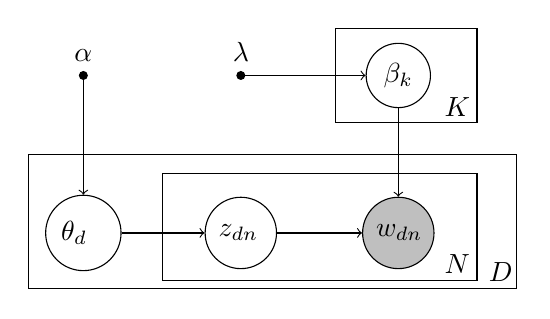
\begin{tikzpicture}
\coordinate (alpha)   at (0,2);
\node (alpha) at (0,2) [circle, draw, inner sep=1pt, fill, label=above:$\alpha$] { };
\node (theta) at (0,0) [circle, draw, text width = 16pt] {$\text{ }\theta_d$};

\node (b) at (2,2) [circle, draw, inner sep=1pt, fill, label=above:$\lambda$] { };
\node (z) at (2,0) [circle, draw, text width = 16pt] {$z_{dn}$};

\node (psis) at (4,2) [circle, draw] {$\beta_k$};
\node (w) at (4,0) [circle, draw, text width = 16pt, fill=gray!50] {$w_{dn}$};

 
\draw[->] (alpha) -- (theta);
\draw[->] (b.east) -- (psis.west);
 
\draw[->] (theta.east) -- (z.west);
\draw[->] (z.east) -- (w.west);
\draw[->] (psis) -- (w);
 
\draw (-0.7,-.7) rectangle (5.5,1);
\draw (1,-.6) rectangle (5,.75);
\draw (3.2,1.4) rectangle (5,2.6);
 
\node at (5.3,-.5) {$D$};
\node at (4.75,-.4) {$N$};
\node at (4.75,1.6) {$K$};
  
\end{tikzpicture}

% ---------------------------------------------------
% Comment below for inclusion in other docs
% ---------------------------------------------------

%\end{document}
        }
        
        
        \begin{align*}
        \thd &\sim \nor{\vv{\mu}}{\Sigma} & \betav_k & \sim \dir{\lambdav} \\
        \zdn &\sim \mulone{\sigma(\thd)} & \wdn & \sim \mulone{\mathbf{\beta}_{z_{dn}}}
        \end{align*}   
    
    \begin{align*}    
        \sigma_k(\vv{\theta}) = \frac{e^{\theta_j}}{\sum_j e^{\theta_j}}
    \end{align*}
    \end{center}
}
\only<3-> {
    Incorporating Link Information: $\Pr(d \rightarrow q) = y_{dq}$
    \begin{description}
        \item<3->[Similarity]\cite{Nallapati2011}: Directly compare topic-distributions
            \only<3>{\begin{align*}
            y_{dq} & \propto \lambda \text{ cos-dist}(\thd, \vv{\theta}_q) \\
                   & + (1-\lambda)  \text{ cos-dist}(\text{tfidf}(\vv{w}_d), \text{tfidf}(\vv{w}_q))
            \end{align*}}
        \item<4->[RTM]\cite{Chang2009a}: Weighted  empirical topic-similarity
            \only<4>{\begin{align*}
                y_{dq} & = \phi \left(\vv{\gamma}\T(\bar{\vv{z}}_d .* \bar{\vv{z}}_q) + \epsilon \right) &
                \bar{\vv{z}}_d & = \frac{1}{N_d}\sum_n \zdn
            \end{align*}}
        \item<5->[LRO]\cite{Neiswanger2014}: Adjusted similarity metric
            \only<5>{\begin{align*}
                y_{dq} & \sim \nor{\gamma \thd\T\vv{\nu}_q}{\tau_{ij}} & \vv{\nu}_{q} & \sim \nor{\vv{\theta}_q}{\lambda I_K}        \end{align*}}

        \item<6->[PLSA+LDA]\cite{Nallapati2008}\cite{Nallapati2008a}: Draw documents from a shared multinomial
        \only<6>{\begin{align*}
            y_{dm} &\sim \mulone{\thd} & l_{dm} & \sim \mulone{\vv{\phi}_{y_{dm}}}
        \end{align*}}
        \item<7>[MMSB]\cite{Gopalan2013b}: Mixed-membership stochastic block-models
    \end{description}
}

\end{frame}


%--- Background ----------------------------------%

\section{Model}

\begin{frame}{Proposed Model - Desiderata}
\begin{itemize}
    \item Avoid learning zeros
    \item Capture difference between out-link and in-link distributions
    \item Try to re-use topic information
    \item Try to incorporate inherent popularity
    \item Use the \emph{incidence} of links as well as presence
    \item Don't address temporal effects
\end{itemize}
\end{frame}

\begin{frame}{Proposed Model}

\only<1->
    \begin{align*}
        \Theta &\sim \mnor{\vv{\mu}\one\T}{\Sigma}{\alpha I_D}&
        \Phi|\Theta   &\sim \mnor{\vv{\Theta}}{\tau I_K}{\diag{\vv{\rho}}}
    \end{align*}
\only<1->
\only<1> {
    \begin{align*}
        A & \sim \mnor{M}{\Sigma}{\Omega} \iff & \vecf{A} & \sim \nor{\vecf{M}}{\Omega \otimes \Sigma} \\
        \mathbb{C}\text{ov}\left[A_{dk}, A_{pj}\right] & = \Omega_{dp} \Sigma_{kj} &
        \mathbb{C}\text{ov}\left[A_{d\cdot}\right] & = \Omega_{dd} \Sigma &
    \end{align*}
}
\only<2> {
    \begin{align*}
        \Phi &\sim \mnor{\vv{\mu}\one\T}{\Sigma + \tau I_K}{\alpha I_D + \diag{\vv{\rho}}}
    \end{align*}
}
\only<3-> {
    \begin{align*}
        z_{dn}|\Theta & \sim \mulone{\sigma(\Theta_{d\cdot})} & 
        w_{dn}|z_{dn},\vv{\beta} & \sim \mulone{\vv{\beta}_{z_{dn}}}
    \end{align*}
}
\only<4-> {
    \begin{align*}
        y_{dm}|\Theta & \sim \mulone{\sigma(\Theta_{d\cdot})} & 
        l_{dm}|z_{dn},\Phi & \sim \mulone{\sigma(\Phi_{\cdot y_{dm}})}
    \end{align*}
}

\end{frame}

\begin{frame}{Bounding the Likelihood: Variational Inference}
We want to incorporate our uncertainty by a lower-bound on the marginal likelihood\cite{WainwrightJordan2008}
\only<1->{
    { \small
    \begin{align*}
    \ln p(W,L) & = \ln \int \int \int \int  p(W , L, \Theta, \Phi, Z, Y , \vv{\beta}) d\Theta d\Phi dZ dY d\vv{\beta} \\
     & \geq \ex{q}{\ln p(W,L, \Theta, \Phi, Z, Y , \vv{\beta})} + \mathbb{H}\left[ q \right]
    \end{align*}
    \normalsize
    }
    Mean-Field Factorisation
    \begin{align*}
    q(\Theta,\Phi,Z,Y,\vv{\beta}) = \prod_k q(\vv{\beta}_k)\prod_d q(\Theta_{d\cdot}) q(\Phi_{d\cdot})\prod_n q(z_{dn}) \prod_m q(y_{dm}) 
    \end{align*}
}
\only<2> {
    \begin{align*}
        q(\Theta_{d\cdot}) &= \mathcal{N}\left(\Theta_{d\cdot}; \mtd, \std \right) &
        q(\Phi_{d\cdot}) &= \mathcal{N}\left(\Phi_{d\cdot}; \mpd, \spd\right) 
    \end{align*}
}
\only<3> {
Maximising this bound is equivalent to minimising the distance to the true posterior
{ \small
\begin{align*}
q \leftarrow \arg \min_q \text{KL}(q(\Theta, \Phi, Z, Y , \vv{\beta})||p(\Theta, \Phi, Z, Y , \vv{\beta}| W,L))
\end{align*}
\normalsize
}
}
\end{frame}

\begin{frame}{Bounding the Log-Sum-Exp function : $\Theta$}
The ELBO still contains an intractable term
\begin{align*}
\ex{q}{p(Z)} & = \sum_d \sum_n \sum_k \zdnk \ex{q}{\Theta_{dk}} 
- \sum_d \ex{q}{\lse{\Theta_{d\cdot}}} \\
\lse{\Theta_{d\cdot}} & = \ln \sum_k \exp(\Theta_{dk})
\end{align*}
Approx via the Bohning Bound\cite{Bohning1988a}
\begin{align*}
\lse{\vv{\thd}} &  \leq \frac{1}{2} \Theta_{d\cdot}\T A \Theta_{d\cdot} - b_d\T \Theta_{d\cdot} + c_d \\
A_K & = \frac{1}{2}(I - \frac{1}{K+1} \one \one\T) \\
b_d & = A_K \xid  - \sigma(\xid) \\
c_d & = \frac{1}{2}\xid\T A \xid  - \sigma(\xid)\T\xid + \lse{\xid}
\end{align*}

\end{frame}

\begin{frame}{Bounding the Log-Sum-Exp function : $\Phi$}
Bohning bound for $\lse{\phok}$ is bounded by $A_D$, $\vv{f}$ and $g$, and can be expressed in terms of $\phdo$. Let $\hat{L}_{dk} = \sum_p \sum_m y_{pmk} l_{pmd}$ and $N^i = \diag{\sum_d \hat{L}_{d\cdot}}$:
\begin{equation*}
\begin{aligned}
p(L|Y) & \geq \sum_k \hat{L}_{\cdot k}\T \phok  - \sum_k N^i_{kk} \left(\half \phok\T A_D \phok - \vv{f}_k\T \phok + g_k\right) \\
& = \Tr{\hat{L} \Phi} - \half \Tr{A_D \Phi N^i \Phi} + \Tr{F \Phi} - \one\T G  \\
& = \sum_d \hat{L}_{d\cdot} \phdo - \half \sum_{p \neq d} A_{dp} \vv{\phi}_{p\cdot}\T N^i \phdo \\
&-\half A_{dd} \phdo\T N^i \phdo + F_{d\cdot}\T\phdo + G_{d\cdot}
\end{aligned}
\end{equation*}

The matrix $F \in \MReal{D}{K}$ and vector $G \in \MReal{1}{K}$ simply collect the vectors $\vv{f}_k$ and scalars $g_k$.

\end{frame}

\begin{frame}{Final Updates}
\small
\begin{align*}
\mtd &= \invb{ \invb{(\alpha + \rho_d)\Sigma} + N^o_d A_K } \\
    & \times
            \left(
                \invb{\rho_d \tau I_K} \mpd
                + \invb{\alpha \Sigma}\vv{\mu}
                + \vv{b}_d 
                + \hat{\vv{z}}_{d\cdot}
                + \hat{\vv{y}}_{d\cdot}
            \right) \\
 \mpd & = \invb{\invb{\rho_d \tau I} + A_{dd}N^i} \\
  & \times
             \left(
                 \invb{\rho_d \tau I}\mtd + N^i F_{d\cdot} -\half \sum_{p \neq d} A_{dp} N^i \vv{m}^\phi_p + \hat{L}_{d\cdot}
             \right)
\end{align*}
\only<1> {
     \begin{align*}
     \ex{q}{z_{dtk}}    & = \frac{\beta_{kt}^{m^\theta_{dk}}}{\sum_j \beta_{jt}^{m^\theta_{dj}}} &
     \beta_{kt} & = \frac{\sum_d w_{dt}\ex{q}{z_{dtk}}}{\sum_v \sum_d w_{dv}\ex{q}{z_{dvk}}} \\
     \vv{\mu} & = \frac{1}{D}\sum_d \mtd &
     \Sigma   & = \frac{1}{D}\sum_d \std + (\vv{\mu} - \mtd)(\vv{\mu} - \mtd)
     \end{align*}
}
\only<2> {
    \begin{align*}
    T & = \exp(M^{\Theta}) &
    U & = T \vv{\beta} \\
    R & = W ./ U &
    \vv{\beta} & = \texttt{normalizerows}(\vv{\beta} .* (T\T R))\\
    \end{align*}
    \begin{align*}
    \vv{\mu} & = \frac{1}{D}\sum_d \mtd &
    \Sigma   & = \frac{1}{D}\sum_d \std + (\vv{\mu} - \mtd)(\vv{\mu} - \mtd)
    \end{align*}
}
\only<3> {
    \begin{align*}
    T & = \exp(M^{\Theta}) &
    U & = T \vv{\beta} \\
    R & = W ./ U &
    \vv{\beta} & = \texttt{normalizerows}(\vv{\beta} .* (T\T R))\\
    \end{align*}
    \begin{align*}
    \rho_d   & = \sum_k S^{\Theta}_{d,kk} + (\mpd - \mtd)\T(\mpd - \mtd)
    \end{align*}
}



    
\normalsize

\end{frame}


%--- Evaluation ----------------------------------%

\section{Evaluation}
\begin{frame}{Evaluation Metrics}

\begin{description}
\item[Mean Reciprocal Rank]: $\frac{1}{D} \sum_d \frac{1}{P} \sum_p \frac{1}{r_p}$, where $r_p$ is the rank of linked document $p$ in the ordered list of links for document $d$ 
\item[Recall at M]: The number of correct links found in the top $m$ links for document $d$ as a proportion of the total number of correct links. 
\item[Precision at M]: The proportion of correct links found in the top $m$ links for document $d$
\item[Mean Average Precision]: Given the ranks of all correct links for a document, average the precision at m for m equal to each of those ranks. 
\end{description}

\end{frame}

\begin{frame}{Evaluation Dataset}

We use the Association for Computational Linguistics (ACL) corpus of academic papers

\begin{itemize}
    \item From which we have extracted link-counts per document
    \item Excluding documents with fewer than three words
    \item Excluding documents with fewer than two out-going links
    \item The corpus consists of 4,264 documents
    \item Having an average of 3,486 words and 11 links
\end{itemize}


\end{frame}

\begin{frame}{Evaluation Results}
\begin{center}
    \includegraphics[scale=0.5]{RPlot.pdf}
\end{center}

\end{frame}

\begin{frame}{Evaluation Results : Comparison}

\begin{center}
    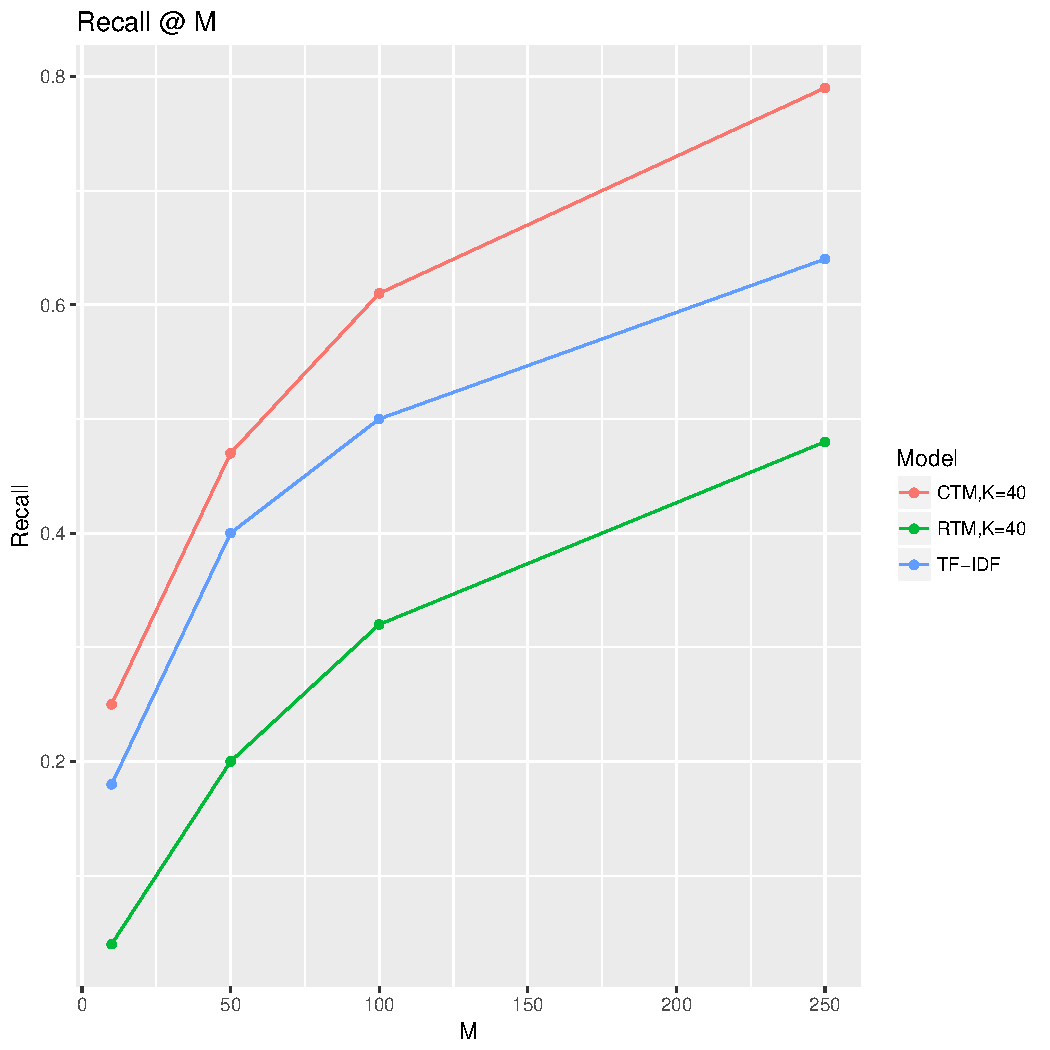
\includegraphics[scale=0.3]{comparison.pdf}
\end{center}

\end{frame}




%--- Questions ----------------------------------%

\section{Conclusions}
\begin{frame}{Conclusions}

We have presented
\begin{itemize}
    \item A model which, for a given paper, can recommend additional within-dataset papers 
    \item Which outperforms RTM and TF-IDF
    \item With an efficient update strategy
    \item Which utilises document/topic information 
\end{itemize}
Further work
\begin{itemize}
    \item Drift over time (e.g. the dynamic topic model \cite{Blei2006a})
    \item Author-to-Author information
\end{itemize}

\end{frame}

\begin{frame}{Conclusions}

Questions?

\end{frame}



%--- the Bibliography frame -------------------------%

\section{References}
\begin{frame}[allowframebreaks]{References}

{\tiny 
    \bibliographystyle{plain}
    \bibliography{/Users/bryanfeeney/Documents/library.bib}
}

\end{frame}



\end{document}
